\documentclass[compress]{beamer}
\usepackage{irbookslide}
\usepackage{irilmenau2}
\usepackage{tikz}
\usepackage{url}
\usepackage{ifxetex}
%\RequireXeTeX
\usepackage{fontspec} % zahteva paket euenc
\usepackage{xunicode}
\usepackage{xltxtra}
\usepackage{polyglossia}
\usepackage{minted}
\usepackage{algorithmic}
\renewcommand{\algorithmicrequire}{\textbf{Input:}}
\renewcommand{\algorithmicensure}{\textbf{Output:}}
\usepackage{xcolor,colortbl}
\usepackage{textcomp}
%\setdefaultlanguage[script=Latin]{serbian}

\title{Stabla}
\author{\textcopyright \ \ Goodrich, Tamassia, Goldwasser}
\institute{Katedra za informatiku, Fakultet tehničkih nauka, Univerzitet u
Novom Sadu}
\date{2014.}
\subject{Predavanja sa ASP}

\begin{document}

\frame{\titlepage}

\section[Pojam]{Pojam stabla}
\begin{frame}[fragile]
  \frametitle{Stablo}
  \begin{itemize}
    \item \myred{stablo} je apstraktni model hijerarhijske strukture 
    \item sastoji se od čvorova koji su u vezi \myred{roditelj}/\myred{dete}
    \item svaki čvor ima najviše jednog roditelja; tačno jedan čvor nema roditelja
    \item čvor ima nula ili više dece
  \end{itemize}
  \begin{center}
    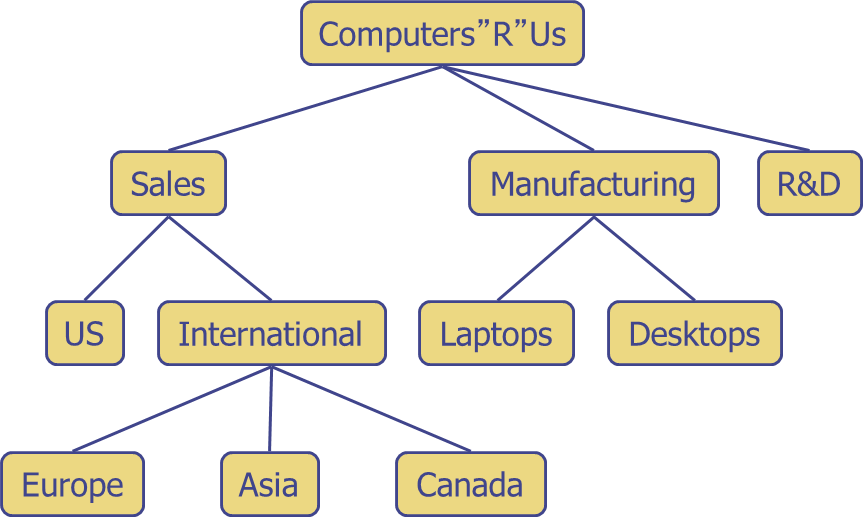
\includegraphics[width=6cm]{asp-08-pic01.png}
  \end{center}
\end{frame}

\begin{frame}[fragile]
  \frametitle{Terminologija}
  \begin{itemize}
    \item \myred{koren} (root): jedini čvor bez roditelja
    \item \myred{unutrašnji čvor}: čvor sa bar jednim detetom
    \item \myred{spoljašnji čvor}/\myred{list} (leaf): čvor bez dece
    \item \myred{predak}: roditelj, deda, pradeda, \ldots do korena
    \item \myred{dubina čvora}: broj predaka
    \item \myred{visina stabla}: najveća dubina
    \item \myred{potomak}: dete, unuče, praunuče, \ldots
    \item \myred{podstablo}: čvor stabla i njegovi potomci
  \end{itemize}
  \begin{center}
    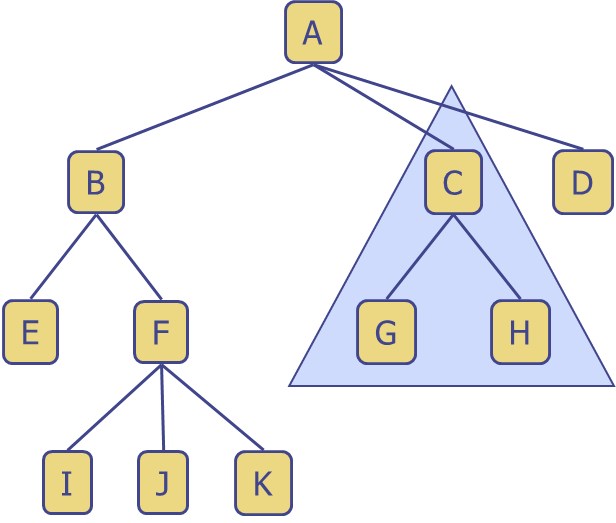
\includegraphics[width=4cm]{asp-08-pic02.png}
  \end{center}
\end{frame}

\begin{frame}[fragile]
  \frametitle{Stablo ATP}
  \begin{itemize}
    \item opšte metode:
    \begin{itemize}
      \item int \myred{len}()
      \item boolean \myred{is\_empty}()
      \item iterator \myred{nodes}()
    \end{itemize}
    \item metode za pristup podacima:
    \begin{itemize}
      \item node \myred{root}()
      \item node \myred{parent}(n)
      \item iterator \myred{children}(n)
      \item int \myred{num\_children}(n)
    \end{itemize}
    \item metode za ispitivanje čvorova:
    \begin{itemize}
      \item boolean \myred{is\_leaf}(n)
      \item boolean \myred{is\_root}(n)
    \end{itemize}
    \item ažuriranje sadržaja:
    \begin{itemize}
      \item element \myred{replace}(n, o)
    \end{itemize}
  \end{itemize}
\end{frame}

\begin{frame}[fragile]
  \frametitle{Stablo u memoriji}
\begin{center}
  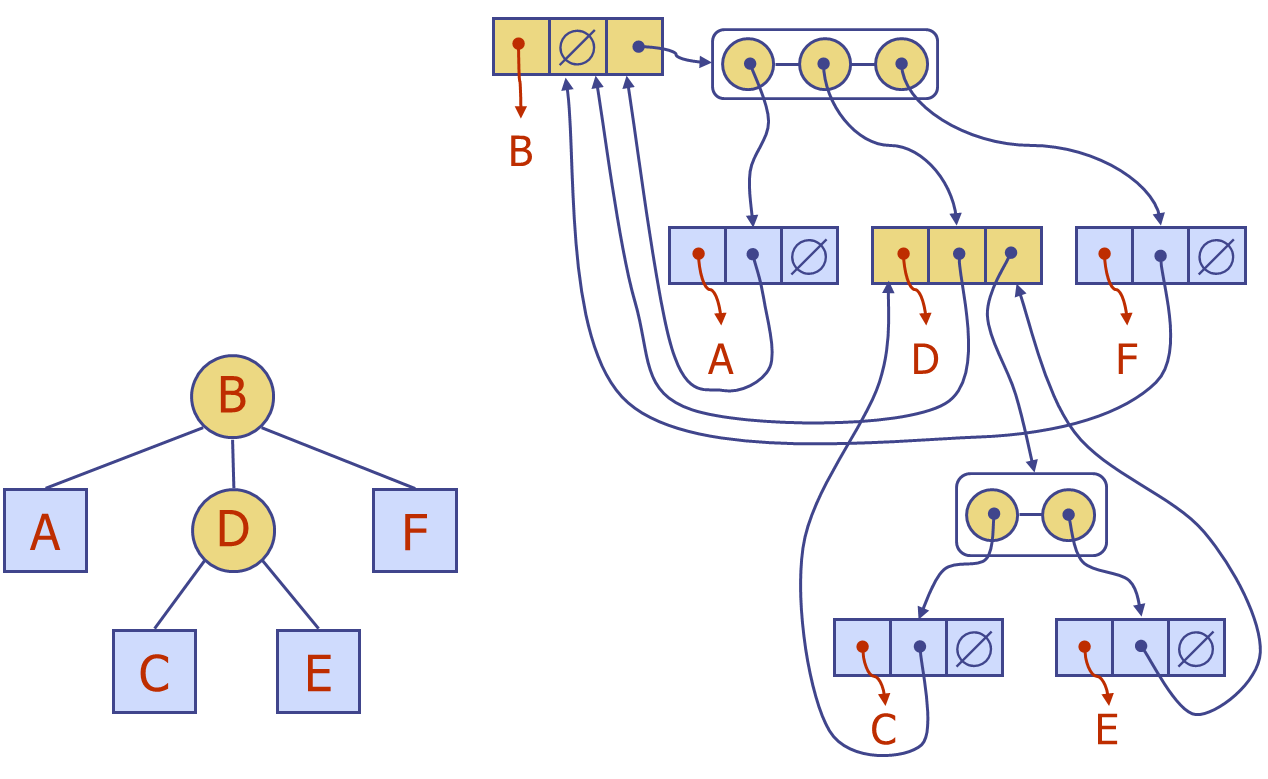
\includegraphics[width=11cm]{asp-08-pic11.png}
\end{center}
\end{frame}

\begin{frame}[fragile,shrink]
  \frametitle{Čvor stabla u Pythonu}
\begin{minted}[linenos=false]{python}
class TreeNode:
  def __init__(self):
    self.element = None
    self.parent = None
    self.children = []
  
  def __eq__(self, other):
    return self == other:
    
  def __ne__(self, other):
    return self != other
  
  def is_root(self):
    return self.parent == None
    
  def is_leaf(self):
    return size(self.children) == 0
\end{minted}
\end{frame}

\begin{frame}[fragile,shrink]
  \frametitle{Stablo u Pythonu $_1$}
\begin{minted}[linenos=false]{python}
class Tree:
  def __init__(self):
    self._root = None
  
  def is_empty(self):
    return self._root == None
    
  def depth(self, node):
    if node.parent is None:
      return 0
    else:
      return 1 + self.depth(node.parent)
\end{minted}
\end{frame}

\section[Obilazak]{Obilazak stabla}
\begin{frame}[fragile]
  \frametitle{Obilazak stabla}
  \begin{itemize}
    \item obilazak \myred{po dubini} (depth-first): obiđi čvor i njegove potomke pre braće
    \begin{itemize}
      \item \myred{preorder}: prvo čvor pa deca
      \item \myred{postorder}: prvo deca pa čvor
    \end{itemize}
    \item obilazak \myred{po širini} (breadth-first): obiđi čvor i njegovu braću pre potomaka
    \begin{itemize}
      \item obilazak ,,po generacijama`` u stablu
    \end{itemize}
  \end{itemize}
\end{frame}

\begin{frame}[fragile]
  \frametitle{Obilazak stabla po dubini / preorder}
\myred{preorder}($n$)
\begin{algorithmic}
\STATE obradi($n$)
\FORALL{dete $c$ od $n$}
  \STATE preorder($c$)
\ENDFOR
\end{algorithmic}
\begin{center}
  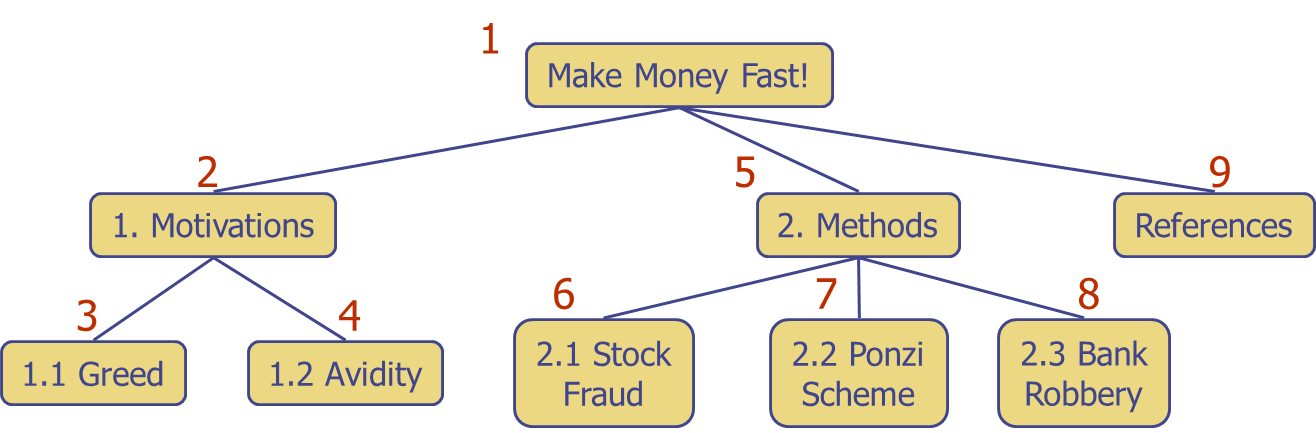
\includegraphics[width=11cm]{asp-08-pic03.png}
\end{center}
\end{frame}

\begin{frame}[fragile]
  \frametitle{Obilazak stabla po dubini / postorder}
\myred{postorder}($n$)
\begin{algorithmic}
\FORALL{dete $c$ od $n$}
  \STATE postorder($c$)
\ENDFOR
\STATE obradi($n$)
\end{algorithmic}
\begin{center}
  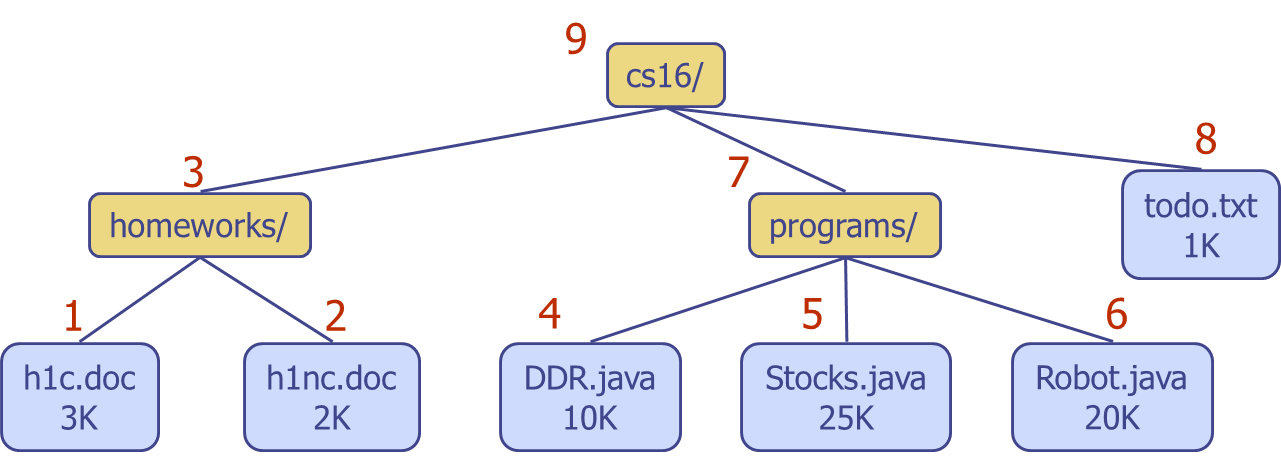
\includegraphics[width=11cm]{asp-08-pic04.png}
\end{center}
\end{frame}

\begin{frame}[fragile,shrink]
  \frametitle{Stablo u Pythonu $_2$}
\begin{minted}[linenos=false]{python}
class Tree:
  ...
  def preorder(self, func):
    self._preorder(self._root, func)
    
  def postorder(self, func):
    self._postorder(self._root, func)
    
  def _preorder(self, node, func):
    func(node)
    for child in node.children:
      self._preorder(child, func)
  
  def _postorder(self, node, func):
    for child in node.children:
      self._postorder(child, func)
    func(node)
\end{minted}
\end{frame}

\begin{frame}[fragile]
\frametitle{Obilazak stabla po širini}
\begin{itemize}
  \item treba obići sve čvorove dubine $d$ pre nego što se pređe na čvorove dubine $d + 1$
  \item primer: stablo igre -- svi mogući ishodi igre koju igra čovek ili računar; koren je početno stanje igre
  \item za igru ,,puta-nula`` (tic-tac-toe)
\end{itemize}
\begin{center}
  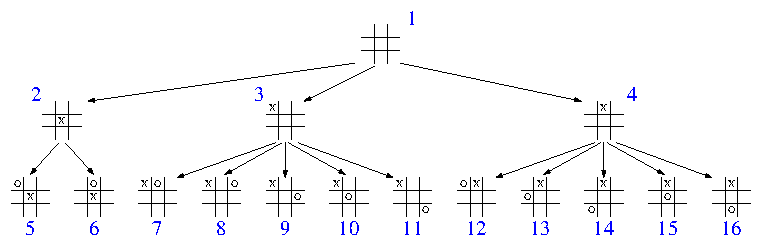
\includegraphics[width=11cm]{asp-08-pic05.pdf}
\end{center}
\end{frame}

\begin{frame}[fragile]
\frametitle{Obilazak stabla po širini}
\begin{columns}
  \begin{column}[c]{6cm}
    \myred{breadth\_first}($root$)
    \begin{algorithmic}
    \STATE napravi novi prazan red $Q$
    \STATE $Q$.add($root$)
    \WHILE{$Q$ nije prazan}
      \STATE $node \leftarrow Q$.dequeue()
      \STATE obradi($node$)
      \FORALL{$child$ dete od $node$}
        \STATE $Q$.enqueue($child$)
      \ENDFOR  
    \ENDWHILE
    \end{algorithmic}
  \end{column}
  \begin{column}[c]{5cm}
    \begin{center}
      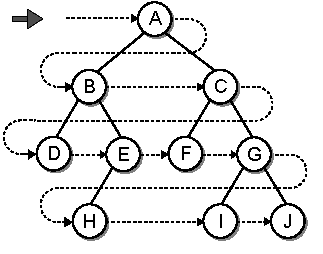
\includegraphics[width=5cm]{asp-08-pic06.pdf}
    \end{center}
  \end{column}
\end{columns}
\end{frame}

\section[2-Stablo]{Binarna stabla}
\begin{frame}[fragile]
  \frametitle{Binarno stablo}
  \begin{itemize}
    \item stablo za koje važi:
    \begin{itemize}
      \item svaki čvor ima najviše dvoje dece
      \item svako dete je označeno kao \myred{levo dete} ili \myred{desno dete}
      \item levo dete po redosledu prethodi desnom detetu 
    \end{itemize}
    \item levo podstablo -- levo dete kao koren
    \item desno podstablo -- desno dete kao koren
    \item \myred{pravilno} binarno stablo: svaki čvor ima 0 ili 2 deteta
  \end{itemize}
  \begin{center}
    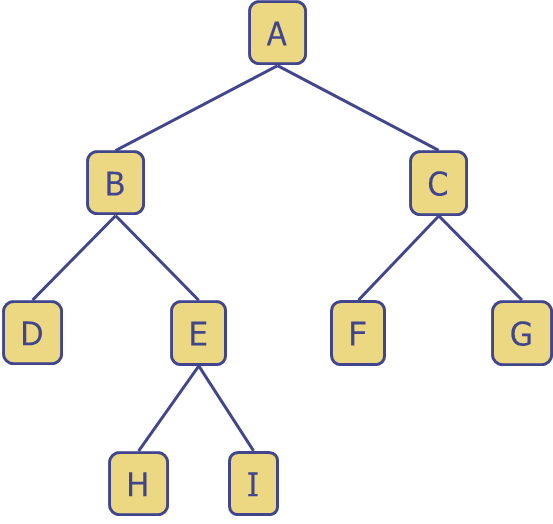
\includegraphics[width=4cm]{asp-08-pic07.png}
  \end{center}
\end{frame}

\begin{frame}[fragile]
  \frametitle{Osobine binarnog stabla}
  \begin{itemize}
    \item nivo stabla $d$ ima najviše $2^d$ čvorova
    \item broj čvorova po nivou raste eksponencijalno
  \end{itemize}
  \begin{center}
    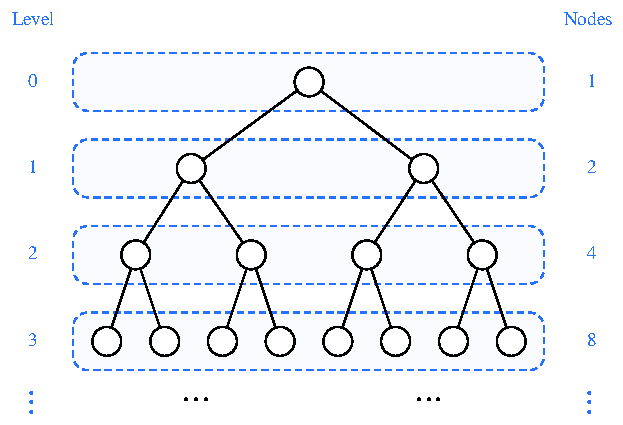
\includegraphics[width=8cm]{asp-08-pic08.pdf}
  \end{center}
\end{frame}

\begin{frame}[fragile]
  \frametitle{Osobine binarnog stabla}
\begin{columns}
  \begin{column}[c]{6cm}
  \begin{itemize}
    \item $n$ -- broj čvorova
    \item $e$ -- broj listova
    \item $i$ -- broj internih čvorova
    \item $h$ -- visina \\ \ \\
    \item $e = i+1$
    \item $n = 2e-1$
    \item $h\leq i$
    \item $h\leq (n-1)/2$
    \item $e\leq 2^h$
    \item $h\geq \log_2 e$
    \item $h\geq log_2(n+1)-1$
  \end{itemize}
  \end{column}
  \begin{column}[c]{5cm}
  \begin{center}
    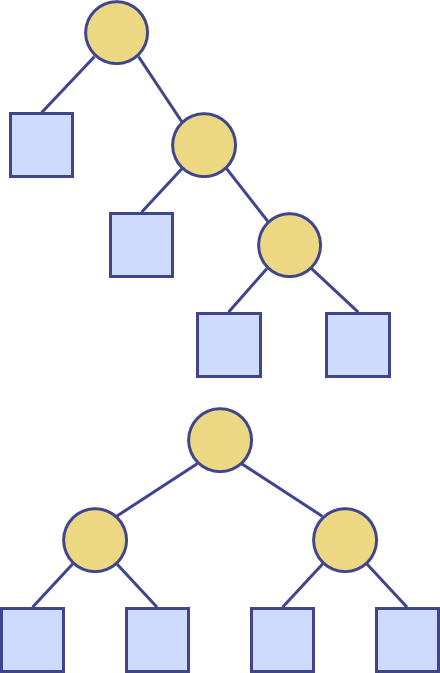
\includegraphics[width=4cm]{asp-08-pic09.png}
  \end{center}
  \end{column}
\end{columns}
\end{frame}

\begin{frame}[fragile]
  \frametitle{Binarno stablo u memoriji / čvorovi i reference}
\begin{center}
  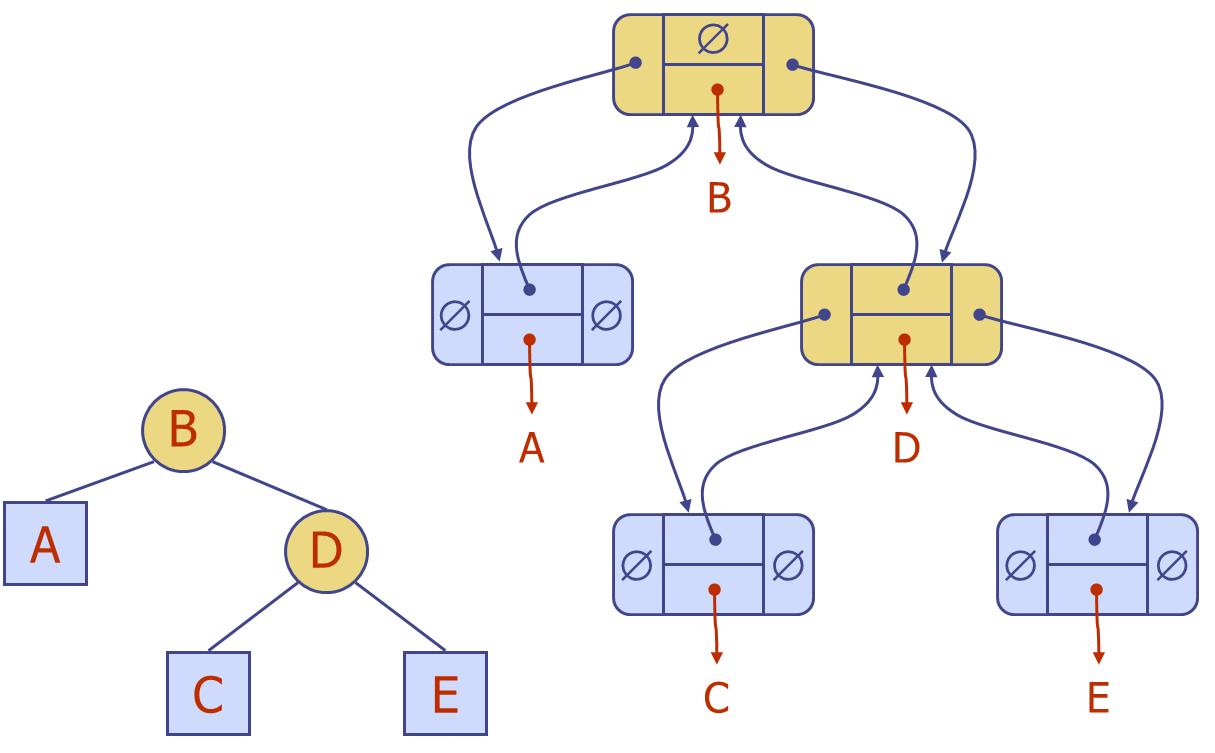
\includegraphics[width=11cm]{asp-08-pic13.png}
\end{center}
\end{frame}

\begin{frame}[fragile]
  \frametitle{Binarno stablo u memoriji / pomoću niza}
\begin{columns}
  \begin{column}[c]{6cm}
  \begin{itemize}
    \item \myred{rang} čvora: 
    \begin{itemize}
      \item $rank(root) = 1$
      \item za levo dete: $rank(node) = 2\cdot rank(parent)$
      \item za desno dete: $rank(node) = 2\cdot rank(parent) + 1$
    \end{itemize}
    \item čvor $v$ se smešta u $A[rang(v)]$
  \end{itemize}
  \end{column}
  \begin{column}[c]{5cm}
  \begin{center}
    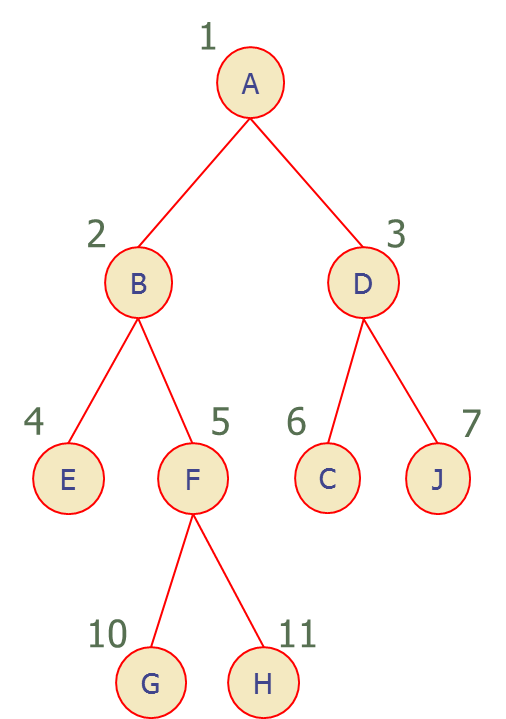
\includegraphics[width=4cm]{asp-08-pic14.png}
  \end{center}
  \end{column}
\end{columns}
\begin{center}
  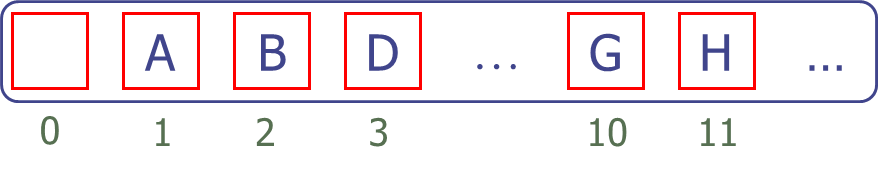
\includegraphics[width=8cm]{asp-08-pic15.png}
\end{center}
\end{frame}

\begin{frame}[fragile]
  \frametitle{Obilazak binarnog stabla / inorder}
\myred{inorder}($n$)
\begin{algorithmic}
\IF{$n$ ima levo dete}
  \STATE inorder(levo dete)
\ENDIF
\STATE obradi($n$)
\IF{$n$ ima desno dete}
  \STATE inorder(desno dete)
\ENDIF
\end{algorithmic}
\begin{center}
  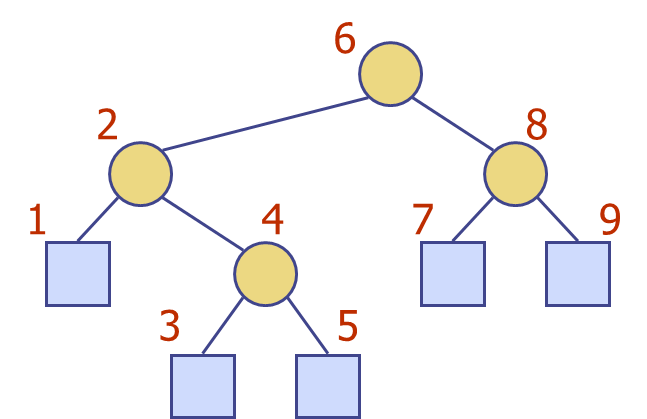
\includegraphics[width=5cm]{asp-08-pic12.png}
\end{center}
\end{frame}

\section[Primeri]{Primeri primene}
\begin{frame}[fragile]
  \frametitle{Stabla odlučivanja}
  \begin{itemize}
    \item binarno stablo strukturirano prema procesu odlučivanja
    \item unutrašnji čvorovi -- pitanja sa da/ne odgovorima
    \item listovi -- odluke
    \item primer: gde za večeru?
  \end{itemize}
  \begin{center}
    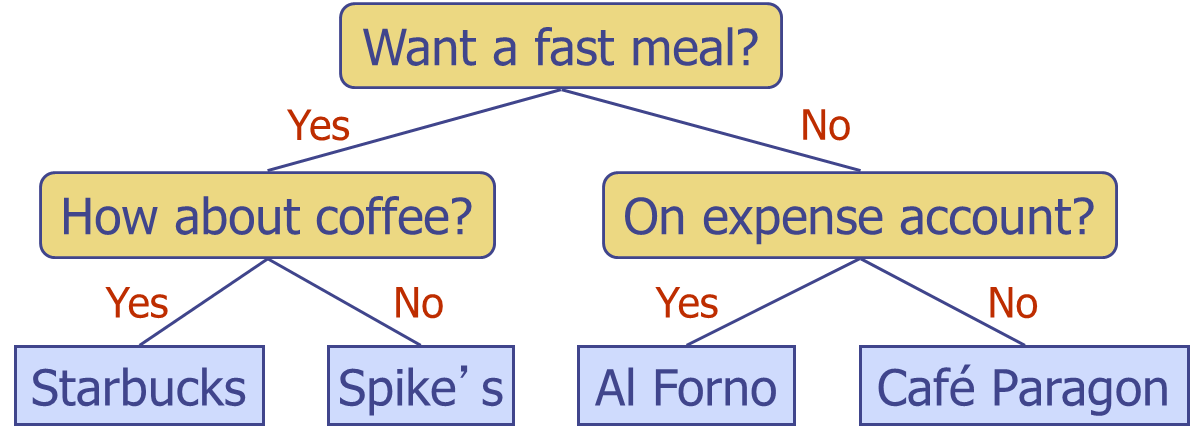
\includegraphics[width=9cm]{asp-08-pic16.png}
  \end{center}
\end{frame}

\begin{frame}[fragile]
  \frametitle{Stablo aritmetičkih izraza}
  \begin{itemize}
    \item binarno stablo kreirano na osnovu aritmetičkog izraza
    \item unutrašnji čvorovi -- operatori
    \item listovi -- operandi
    \item primer: $2 * (a - 1) + 3 * b$
  \end{itemize}
  \begin{center}
    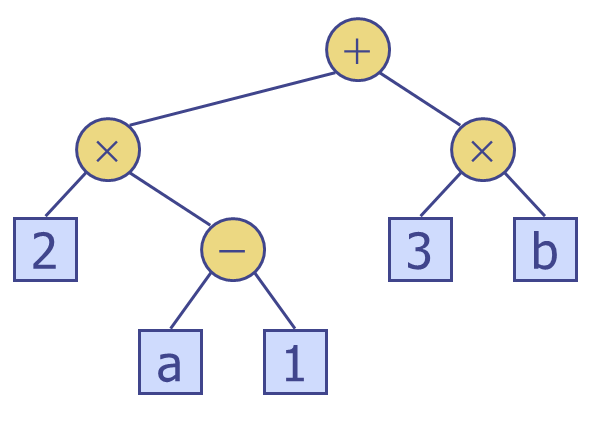
\includegraphics[width=6cm]{asp-08-pic10.png}
  \end{center}
\end{frame}

\begin{frame}[fragile]
  \frametitle{Ispisivanje aritmetičkih izraza}
  \begin{itemize}
    \item specijalni slučaj \textbf{inorder} obilaska
  \end{itemize}
\begin{columns}
  \begin{column}[c]{5cm}
    \myred{printExpr}($n$)
    \begin{algorithmic}
    \IF{$n$ ima levo dete}
      \STATE print("(")
      \STATE printExpr(levo dete)
    \ENDIF
    \STATE print($n$)
    \IF{$n$ ima desno dete}
      \STATE printExpr(desno dete)
      \STATE print(")")
    \ENDIF
    \end{algorithmic}
  \end{column}
  \begin{column}[c]{6cm}
    \begin{center}
      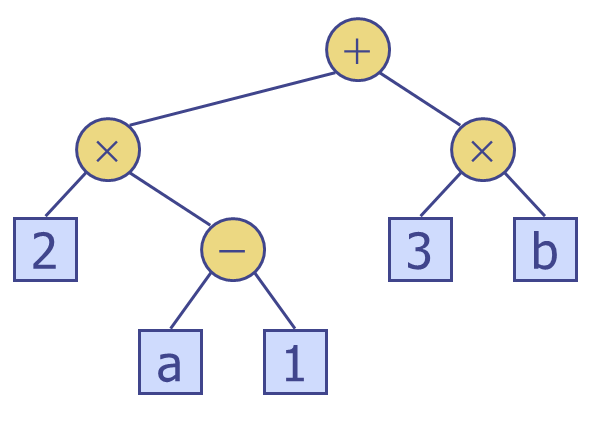
\includegraphics[width=6cm]{asp-08-pic10.png}
    \end{center}
  \end{column}
\end{columns}
\end{frame}

\begin{frame}[fragile]
  \frametitle{Izračunavanje aritmetičkih izraza}
  \begin{itemize}
    \item specijalni slučaj \textbf{postorder} obilaska
  \end{itemize}
\begin{columns}
  \begin{column}[c]{5cm}
    \myred{evalExpr}($n$)
    \begin{algorithmic}
    \IF{$n$ je list}
      \RETURN $n$.$element$
    \ELSE
      \STATE $x \leftarrow evalExpr(n.left)$
      \STATE $x \leftarrow evalExpr(n.right)$
      \STATE $\diamond \leftarrow$ operator u $n$
      \RETURN $x \diamond y$
    \ENDIF
    \end{algorithmic}
  \end{column}
  \begin{column}[c]{6cm}
    \begin{center}
      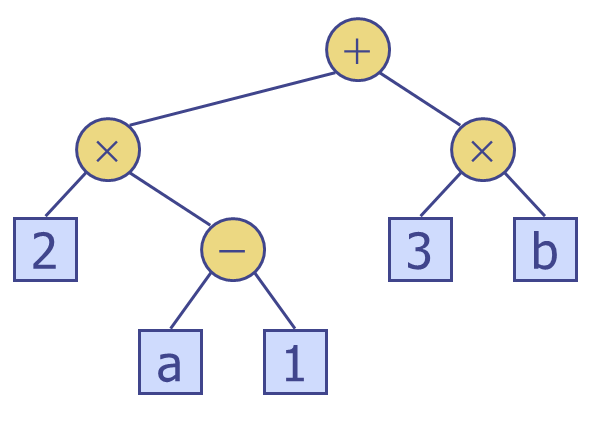
\includegraphics[width=6cm]{asp-08-pic10.png}
    \end{center}
  \end{column}
\end{columns}
\end{frame}

\begin{frame}[fragile]
  \frametitle{Ojlerov obilazak stabla}
  \begin{itemize}
    \item opšti postupak za obilazak stabla
    \item preorder, inorder, postorder su specijalni slučajevi
    \item posmatramo grane stabla kao zidove koji uvek moraju da nam budu sa leve strane prilikom kretanja
    \item svaki čvor se poseti tri puta
    \begin{itemize}
      \item sa leve strane (preorder)
      \item sa donje strane (inorder)
      \item sa desne strane (postorder)
    \end{itemize}
  \end{itemize}
  \begin{center}
    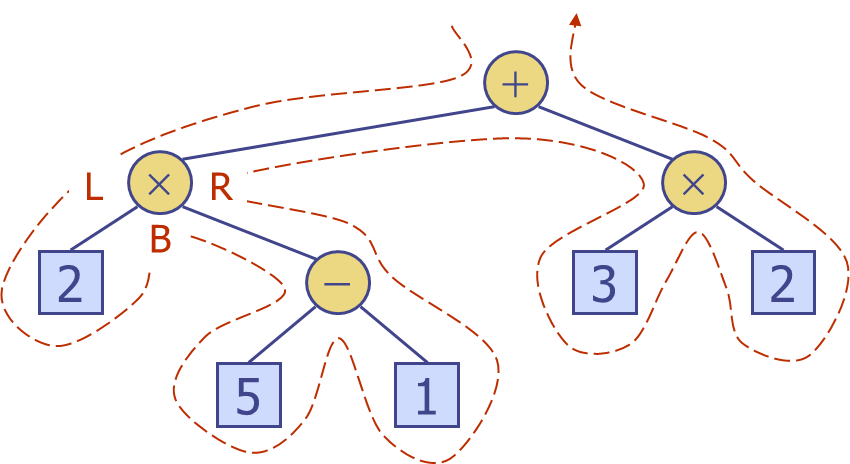
\includegraphics[width=6.5cm]{asp-08-pic17.png}
  \end{center}
\end{frame}

\begin{frame}[fragile]
  \frametitle{Crtanje stabla}
  \begin{itemize}
    \item treba odrediti $(x,y)$ koordinate čvorova stabla
    \item $x(n)$: broj čvorova posećenih pre čvora $n$ u \textbf{inorder} obilasku
    \item $y(n)$: dubina čvora $n$
  \end{itemize}
  \begin{center}
    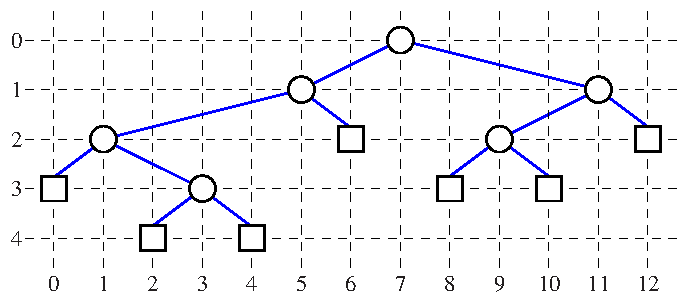
\includegraphics[width=10cm]{asp-08-pic18.pdf}
  \end{center}
\end{frame}

\end{document}
